%%
%% This is file `sample-manuscript.tex',
%% generated with the docstrip utility.
%%
%% The original source files were:
%%
%% samples.dtx  (with options: `all,proceedings,bibtex,manuscript')
%% 
%% IMPORTANT NOTICE:
%% 
%% For the copyright see the source file.
%% 
%% Any modified versions of this file must be renamed
%% with new filenames distinct from sample-manuscript.tex.
%% 
%% For distribution of the original source see the terms
%% for copying and modification in the file samples.dtx.
%% 
%% This generated file may be distributed as long as the
%% original source files, as listed above, are part of the
%% same distribution. (The sources need not necessarily be
%% in the same archive or directory.)
%%
%%
%% Commands for TeXCount
%TC:macro \cite [option:text,text]
%TC:macro \citep [option:text,text]
%TC:macro \citet [option:text,text]
%TC:envir table 0 1
%TC:envir table* 0 1
%TC:envir tabular [ignore] word
%TC:envir displaymath 0 word
%TC:envir math 0 word
%TC:envir comment 0 0
%%
%%
%% The first command in your LaTeX source must be the \documentclass
%% command.
%%
%% For submission and review of your manuscript please change the
%% command to \documentclass[manuscript, screen, review]{acmart}.
%%
%% When submitting camera ready or to TAPS, please change the command
%% to \documentclass[sigconf]{acmart} or whichever template is required
%% for your publication.
%%
%%

\documentclass[screen,review]{acmart}

\usepackage{geometry}
\geometry{%
  left=3cm,right=3cm,
  top=80pt,bottom=80pt, % <===============================================
  headsep=10pt,
  a4paper,
}

%%
%% \BibTeX command to typeset BibTeX logo in the docs
\AtBeginDocument{%
  \providecommand\BibTeX{{%
    Bib\TeX}}}

%% Rights management information.  This information is sent to you
%% when you complete the rights form.  These commands have SAMPLE
%% values in them; it is your responsibility as an author to replace
%% the commands and values with those provided to you when you
%% complete the rights form.


%%
%%  Uncomment \acmBooktitle if the title of the proceedings is different
%%  from ``Proceedings of ...''!
%%
%%\acmBooktitle{Woodstock '18: ACM Symposium on Neural Gaze Detection,
%%  June 03--05, 2018, Woodstock, NY}


%%
%% Submission ID.
%% Use this when submitting an article to a sponsored event. You'll
%% receive a unique submission ID from the organizers
%% of the event, and this ID should be used as the parameter to this command.
%%\acmSubmissionID{123-A56-BU3}

%%
%% For managing citations, it is recommended to use bibliography
%% files in BibTeX format.
%%
%% You can then either use BibTeX with the ACM-Reference-Format style,
%% or BibLaTeX with the acmnumeric or acmauthoryear sytles, that include
%% support for advanced citation of software artefact from the
%% biblatex-software package, also separately available on CTAN.
%%
%% Look at the sample-*-biblatex.tex files for templates showcasing
%% the biblatex styles.
%%

%%
%% The majority of ACM publications use numbered citations and
%% references.  The command \citestyle{authoryear} switches to the
%% "author year" style.
%%
%% If you are preparing content for an event
%% sponsored by ACM SIGGRAPH, you must use the "author year" style of
%% citations and references.
%% Uncommenting
%% the next command will enable that style.
%%\citestyle{acmauthoryear}
\usepackage{listings}
\usepackage{xcolor}

\colorlet{punct}{red!60!black}
\definecolor{background}{HTML}{FFFFFF}
\definecolor{delim}{RGB}{20,105,176}
\colorlet{numb}{magenta!60!black}

\lstdefinelanguage{json}{
    basicstyle=\normalfont\ttfamily,
    numbers=left,
    numberstyle=\scriptsize,
    stepnumber=1,
    numbersep=8pt,
    showstringspaces=false,
    breaklines=true,
    frame=lines,
    backgroundcolor=\color{background},
    literate=
     *{:}{{{\color{punct}{:}}}}{1}
      {,}{{{\color{punct}{,}}}}{1}
      {\{}{{{\color{delim}{\{}}}}{1}
      {\}}{{{\color{delim}{\}}}}}{1}
      {[}{{{\color{delim}{[}}}}{1}
      {]}{{{\color{delim}{]}}}}{1},
}

%%
%% end of the preamble, start of the body of the document source.
\begin{document}


%%
%% The "title" command has an optional parameter,
%% allowing the author to define a "short title" to be used in page headers.
\title[etcd]{\textit{etcd} \\
A key-value NoSQL solution for distributed systems }

%%
%% The "author" command and its associated commands are used to define
%% the authors and their affiliations.
%% Of note is the shared affiliation of the first two authors, and the
%% "authornote" and "authornotemark" commands
%% used to denote shared contribution to the research.
\author{Fábio Sá}
\email{up202007658@fe.up.pt}
\affiliation{%
  \institution{FEUP}
  \city{Porto}
  \country{Portugal}
}

\author{Inês Gaspar}
\email{up202007210@fe.up.pt}
\affiliation{%
  \institution{FEUP}
  \city{Porto}
  \country{Portugal}
}

\author{José A. Gaspar}
\email{up202008561@fe.up.pt}
\affiliation{%
  \institution{FEUP}
  \city{Porto}
  \country{Portugal}
}


%%
%% By default, the full list of authors will be used in the page
%% headers. Often, this list is too long, and will overlap
%% other information printed in the page headers. This command allows
%% the author to define a more concise list
%% of authors' names for this purpose.
\renewcommand{\shortauthors}{F. Sá, I. Gaspar, J. A. Gaspar}

%%
%% The abstract is a short summary of the work to be presented in the
%% article.
\begin{abstract}
The present report aims to explore, both theoretically and practically, the \textit{etcd} technology, a non-relational database using key-value paradigm.
Throughout the document, characteristics of the technology are presented, as well as its specificities and use cases. Next, a specific scenario is addressed, along with the strategies supporting the solution found. Finally, the implementation of the prototype using \textit{etcd} is explained, considering the aforementioned ideation, \textit{etcd} characteristics and some considerations of features in this paradigm.
\end{abstract}


%%
%% Keywords. The author(s) should pick words that accurately describe
%% the work being presented. Separate the keywords with commas.
\keywords{NoSQL, \textit{etcd}, Key-Value, consistency, distributed systems, full replicated}

%%
%% This command processes the author and affiliation and title
%% information and builds the first part of the formatted document.
\maketitle

\section{Introduction}
The increase in the amount of data and the complexity of systems has led to the creation of new database solutions, non-relational databases \cite{nosql}, with the aim of providing efficient storage and retrieval of data and allowing rapid access in large-scale applications. \\
In this way, various paradigms have emerged, including key-value, which is explored in this report.
This approach has a very simple design, since it only depends on the design of the key and most of the processing and manipulation required is on the application side. These NoSQL technologies allow for great scalability and better time performance than relational databases. They are therefore often used as caching systems, where data is temporarily stored for quick access. However, the use of these strategies can lead to a problem known as \textit{Impedance Mismatch} \cite{impedance}, i.e. discrepancies between the models of the structure of the technology used in the application and the model used in the database.
\textit{etcd}  is a database often used for setting up distributed systems. It is especially used because of the strong consistency between nodes that it allows, which will be explored in the following sections, as well as through the use cases of this technology and the prototype developed.
    
    
\section{Technology}
In this section, \textit{etcd} is going to be described in terms of features, data model, advantages, limitations an some use cases are also presented.

\subsection{Overview}
\textit{etcd} is a distributed key-value database \cite{key}. Key-value databases are a type of NoSQL database paradigm that stores data as a collection of key-value pairs, where each key is unique and associated with a single value.
This database system was initially developed by CoreOS \cite{core} in 2013, when it had its first release. In 2018, RedHat \cite{red} announced the acquisition of CoreOS, and IBM \cite{ibm} announced the acquisition of RedHat in the same year.
\textit{etcd} is free and follows an open-source licensing model. Its official documentation \cite{documentation} features many tutorials, demos, and installation instructions, as well as an extensive FAQ \cite{etcd_faq}. The community \cite{com} is active and supportive, with user and developer forums on Google Groups \cite{google}, real-time updates on Twitter \cite{twitter}, and discussions on GitHub \cite{github}. Additionally, contributors and maintainers hold weekly online meetings via Zoom, with meeting documentation available and sessions archived on YouTube. As of the date of this report, it ranks 54th among the most used database engines and 5th in the key-value paradigm, according to the evaluation on db-engines.com \cite{db-engines}.

The name "etcd" originated from two ideas: the Unix "/etc" folder and "d"istributed systems \cite{dbdb}. The "/etc" folder is a place to store configuration data for a single system, whereas \textit{etcd} stores configuration information for large-scale distributed systems. Thus, it is widely used for configuration management, service discovery, and coordination in distributed systems.

\textit{etcd} provides a reliable way to store data across a cluster of machines and ensures strong consistency guarantees. Unlike most other NoSQL databases, \textit{etcd} is designed to be highly available and fault-tolerant, making it a popular choice for storing data in distributed systems \cite{ibm} \cite{etcd_overview}. As specified by the CAP theorem \cite{ibm_CAP} (Consistency, Availability, Partition Tolerance), in order to achieve strong consistency, \textit{etcd} sacrifices performance, which makes it not ideal for projects where execution time is crucial.

\subsection{ACID Properties}
\textit{etcd} guarantees the ACID properties \cite{acid} (Atomicity, Consistency, Isolation, and Durability) within transactions. However, they only exist for one key-value set, i.e. it is not possible to change more than one key-value pair in a transaction \cite{transaction}.
A transaction is an atomic If/Then/Else construction on key-value pairs. They are often used to protect keys from unintentional concurrent updates, create compare and exchange operations and develop better higher-level concurrency control.
They can atomically process several requests in just one. Each change to a key-value pair causes the revision (the version of a given key-value pair) to be added for the given transaction, as well as all the events triggered by the transaction being part of the same revision. However, it is not allowed to change the same key several times in a single transaction.
Transactions are protected by comparisons, i.e. each of these comparisons checks a single key from those stored. In this way, they work by checking the absence or presence of a value and comparing it with a given one, or by checking the revisions. In terms of comparisons, two different ones can be applied to the same key or to different keys.
These are applied atomically as follow: if all the comparisons are true, then the transaction was successful and \textit{etcd} executes the then (success) request block for the transaction, otherwise it is said to have failed and the else (failure) request block is executed.


\subsection{Features}

As it is going to be described throughout this section, \textit{etcd} has several features, some of them unique, that make this database a good choice in many distributed systems.\\

\subsubsection{Replication and node communication features}~\

This database is built to work in a distributed way \cite{etcd_clustering}, when the number of nodes / machines is greater than one. This cluster can be generated through an internal network between several nodes. In \textit{etcd} the number of nodes is preferably odd for resource management purposes.

\textit{etcd}  is built on the Raft consensus algorithm \cite{raft} to ensure data store consistency across all nodes in a cluster for a fault-tolerant distributed system. This algorithm is based on quorums and as the name suggests it is used to have a consensus between a majority of nodes about the values that are being stored in the database, taking into account that one or more nodes may fail. In \textit{etcd}, for a cluster with N members, the quorum size is (N/2)+1. For any odd-sized cluster, adding one node will always increase the number of nodes necessary for quorum.

These nodes do not need to be physically together, even though it may affect request latency. \textit{etcd} stablishes connection between nodes via HTTP + TLS \cite{http}. If the IP of the node is not known, \textit{etcd} has a discovery mode that will find the node's IP address and establish the connection.
In terms of load balancing, it is usefull to state that there is a leader node. This node is responsible for ensuring data replication among non-leader nodes and balance the distribution of request among those nodes \cite{etcd_faq}.
Even though it is possible to have multiple nodes in one cluster, \textit{etcd} does not provide a way to support multiple clusters that can communicate with each other. To implement that feature, some communication protocol must be implemented between the clusters. One possible approach would be to put the leader node of each cluster in charge of that communication.

Each node has a copy of the data, and the data is replicated across the cluster. This means that, if a node fails, the data is still available on the other nodes, even if the leader is down - reelection is done. As such, having a leader does not represent a critical point of failure for the system. It only fails if the majority of nodes are down, that is, consensus is not obtained.
In \textit{etcd} there is a total replication of the data between all nodes, which means, it's full replicated. \\

\subsubsection{Consistency features}~\

\textit{etcd} provides sequential consistency, which is the stronger form of consistency that can be obtained in distributed systems. This means that, independently of the node of the cluster that receives the request from the client, it reads the same events in the same order.

Note that eventual consistency is not enough, specially in critical systems where, if in any moment, there are inconsistent states on the nodes, since they probably have configurations of systems stored in it - main purpose of \textit{etcd} - it can cause critical problems to the systems, making it, for example, vulnerable to some mallicious attacks.

It's also important to mention that, each key has a version that is required internally to achieve consistency in the distributed system and \textit{etcd} allows users to see those versions and the respective values.

Consistency is one of the advantages of using a distributed database. It allows for multiple nodes to be updated at the same time, which can lead to inconsistencies in the data. To avoid this, \textit{etcd} provides a quorum like strategy, which ensures that the data is consistent across all nodes in the cluster even if some nodes are down at that given moment\cite{etcd_api}. \\

\subsubsection{Watcher feature}~\

\textit{etcd} provides a functionality called Watcher \cite{etcd_watcher}. This watcher can be used to monitor a given value of a certain key over time based on the operations executed over that key-value pair.

It's possible to specify whether to monitor only the PUT, only the GET operations, or both, depending on the problem.
With this feature it can be seen how useful this database is regarding system configurations. With this monitoring feature it is extremely easy to see modifications in critical variables in real-time (without resort to polling), helping to prevent any unwanted results. \\

\subsubsection{Data processing features}~\

Regarding data processing features, \textit{etcd} provides a limited range of those. As an example, functions like counts, sums, averages, map-reduces that are supported by other databases have no translation in \textit{etcd}, making mandatory to process information after querying the database or designing key-value structures in a way to make post-processing unnecessary.
As it can be seen in the oficial documentation of \textit{etcd}, the main supported features are methods to read, write and delete data, besides the ability to monitor changes in a given key-value pair plus the possibility of knowing the version of the key and seeing old values for a given key \cite{etcd_interacting} \cite{etcd_api}.

However, it is not only in data processing features that \textit{etcd} is not ideal, also on the data types that can be stored in \textit{etcd}. These types consist in strings and numbers, so there are no lists, sets or more complex data types. \\

\subsubsection{Prefix feature}~\

\textit{etcd} has another peculiar feature that can be very handy, the prefix search. This feature allows users to search for a range of keys based on the prefix. Since \textit{etcd} is fully replicated, it is possible to obtain all the keys with the same prefix only performing one request to exactly one node of the cluster, making this operation efficient.
To exemplify this feature, if the keys \textbf{app:foo} and \textbf{app:bar} exist, the prefix \textbf{app:} can be used to retrieve both keys and their respective values.

\subsection{CLI and Client libraries}

\textit{etcd} provides a CLI, etcdctl \cite{etcd_clt}. Currently in version 3, this command line interface allows interacting with the database at a lower level. It's a wrapper for the documented API.

Due to its widespread use, \textit{etcd} is combined with various open-source libraries \cite{etcd_library}, ensuring a suitable interface between \textit{etcd} clusters and the backend of applications that use this technology. Examples include Microsoft's etcd3 \cite{etcd_microsoft}, suitable for Javascript and Typescript, and Python-etcd3 \cite{etcd_python} for Python.

\subsection{Data Model}
The data model \cite{etcd_data_model} can be seen logically and physically. Throughout this section both of them are going to be described. \\

\subsubsection{Logical View}~\\
The database's logical view is a flat binary key space with a lexically sorted index for efficient range queries. It maintains multiple revisions, with each atomic mutative operation creating a new revision. Old revisions of keys remain accessible through previous revisions, and they are indexed for efficient ranging. Revisions are monotonically increasing over time.

A key's life spans a generation from creation to deletion, with each key having one or multiple generations. Creating a key increments its version, starting at 1 if it doesn't exist. Deleting a key generates a tombstone, resetting its version to 0. Each modification increments a key's version within its generation. \\

\subsubsection{Physiscal View}~\\
\textit{etcd} stores data in a persistent B-Tree \cite{b-tree}, with each revision containing only the delta from the previous one for efficiency reasons. Keys are represented as 3-tuples (major, sub, type), allowing differentiation and optional special values like tombstones. The B-Tree is ordered lexically for fast ranged lookups over revision deltas. Compaction removes outdated key-value pairs. Additionally, \textit{etcd} maintains an in-memory B-Tree index for speedy range queries, with keys exposed to users and pointers to modifications in the persistent B-Tree.

\subsection{Supported Data Operations}
\textit{etcd} provides an HTTP/JSON API \cite{etcd_api} that allows clients to perform CRUD operations \cite{crud} on the database.
There are mainly 2 operations, GET and PUT. As the names suggest, these operations are used to retrieve a given value based on a key and store a new or an existent key-value pair, respectively. 
Regarding updates, they are just a new PUT, over the same key.
It is also possible to delete key-value pairs using the delete operation.
Another interesting feature provided by the API is the ability to check the cluster' health. Parameters like the leader node and the number of requests can be seen via this API.
Regarding the watchers, via the API, it is possible to create them and generate a function that is going to run at each operation over the key that is being monitored \cite{etcd_api}.

\subsection{Use Cases}
As previously mentioned, \textit{etcd} is used mainly to perform system configurations in distributed systems \cite{etcd_why}.
The most important use cases are:

\begin{itemize}
    \item Kubernetes \cite{kubernetes} - Uses \textit{etcd} to store all its data – its configuration data, its state, and its metadata. 
    \item Container Linux by CoreOS \cite{coreos} - Uses \textit{etcd} to store the configuration data of their internal distributed system.
\end{itemize}

\subsection{Problematic Scenarios}

One of the problematic scenarios of \textit{etcd} is related with the restricted data types that can be stored in the database. Only numbers and strings are accepted. There is a need to keep a json encoded as string when more complex types are required and the attribute search over the value is impossible: the system must receive the entire entity and then select the attribute manually.

\textit{etcd} was developed to deal with small key-value pairs, typically designed to metadata. Hence, the maximum size of any request is 1.5 MiB. Similarly, the suggested maximum size of the database is 8 GiB (2 GiB is the default). This database was not built to be used as a cache, as most key-value databases\cite{etcd_sys_limits}, since the data is allocated in the hard-disk.

Fast disks are vital for \textit{etcd} performance and stability \cite{etcd_hw}. Slow disks increase request latency and cluster instability. \textit{etcd}'s consensus protocol requires timely storage of metadata to a log, with most cluster members writing every request to disk. \textit{etcd} also checkpoints its state to disk for log truncation, and delays in these writes can cause heartbeat timeouts, triggering cluster elections and instability. \textit{etcd} is highly sensitive to disk write latency, needing at least 50 sequential IOPS (e.g., from a 7200 RPM disk) and ideally 500 sequential IOPS (e.g., from a local SSD or high-performance virtualized block device) for heavily loaded clusters. This limitation, together with the inability of writting a block of key-value pairs in one operation - would eventually surpass the 1.5MiB of request - makes the entire cluster slower when facing lots of consecutive writes. This drawback is noticeable when populating an \textit{etcd} database for example.

Furthermore, \textit{etcd} can also become problematic due to its own nature of replicating data totally. It is possible to have several nodes running to ensure data is (almost) never lost, however this makes the entire system slower with the increase of nodes, precisely due to data consistency and replication.

\subsection{\textit{etcd} vs. Other Solutions}
As previously mentioned, \textit{etcd} is not like most key-value databases. It is recommended to be used when sequential consistency is needed, in distributed systems, and not to be used as a cache, like Redis \cite{redis}, for example. There is a tradeoff between having a fast response time and having a consistent state. \textit{etcd} is made not to be fast but consistent while most key-value databases are made to be fast but not consistent.
The main advantage of \textit{etcd} is the ability of having more than one point of failure. Thanks to the Raft consensus algorithm, if more than 50\% of the nodes are up and running, the system will be able to continue working and accept new operations over the database. Then, when the nodes that fail recover, the state is fully replicated to those nodes achieving the sequential consistency that is needed and guaranteed by the API.
Other advantage, as specified in \textit{etcd} documentation, is the maximum reliable database size.\textit{etcd} can scale up to several gigabytes while others (e.g ZooKeeper \cite{zoo} and Consul \cite{consul}) can only support scalable results until hundreds of megabytes.
The main drawback is the performance of \textit{etcd} and the lack of ability of inserting larges amount of data in a block. Operations on database are restrict to one at a time.

\section{Prototype}
To validate the main features, qualities, and potential bottlenecks of the mentioned \textit{etcd} technology, a prototype — proof of concept based on this key-value paradigm — was developed and presented in the following sections.

\subsection{Topic}
In a classic scenario of purchasing tickets for events, data consistency is the most important aspect to consider. For example, each event should display its updated information in real-time, including the number of remaining tickets, regardless of the number of simultaneous purchases occurring. A failure in data replication and propagation within the system can result in event overbooking, inaccurately computed purchases, and potential revenue loss.

To ensure the system is immune to such issues, it is necessary to rely on a database that is simultaneously:

\begin{itemize}
    \item Distributed, for horizontal scalability ensuring the system can handle the growing workload effectively;
    \item Fully replicated, where every data read returns the latest data write across all clusters and nodes, something that is not achievable with eventual consistency;
    \item Highly available, to have no single point of failure and gracefully tolerate hardware failures and network partitions.
\end{itemize}

TickETCD, a web application for purchasing tickets for events, uses \textit{etcd} as a solution to the aforementioned problems. The implementation details will be described in the following subsections.

\subsection{Dataset}
Given the unavailability of data of this nature suitable for the application, TickETCD's data is generated using the Python Faker Library \cite{faker} and a configuration file. Among other factors, this stage allows for changing the number of created users, the number of events, the probability of a user being an administrator, the probability of creating and triggering a notification, choosing locations and event types, as well as ticket types and price ranges.

These configurations are important to establish a system governed by scalable and parameterizable data. Although the data is invented and probabilistic, it is also reliable, adapted, and aligned with reality.

\subsection{Conceptual Data Model}
In order to meet the needs of the application, the following relationships have been designed, as shown in Figure \ref{fig:UML}.

An event has a name, location, date, type, description, and a total quantity of available tickets. Each event may offer various ticket types, each associated with a price, as well as their initial and current total quantity. Users, identified by their name, email, password, and role, can have favorite events and request notifications when the quantity of tickets for a specific event reaches a certain limit. Additionally, users can purchase various types of tickets.

\subsection{Physical Data Model and Data Structures}
The previous Conceptual Data Model could be implemented physically using relational database schemas, allowing for direct searches for relationships between entities. However, in the case of dealing with the key-value paradigm used in \textit{etcd}, it was necessary to resort to data redundancy to ensure complete knowledge of all relationships and still minimize the number of post-processing steps.

Below are presented the key and value structures and aggregates used for the design of the entire data structure required by TickETCD. It should be noted that for the purpose of data visualization and manipulation, JSON was used, although physically, they are just strings after serialization, as \textit{etcd} does not support other data types as values for its keys. \\

\subsubsection{User}~\\
Without any post-processing, it is possible to query all information related to a user by querying the key in the format \textbf{user:<USERNAME>}. Example:

\begin{lstlisting}[language=json]
"user:johndoe": { 
    "name": "jonh doe", "email": "john@mail.com", 
    "password": "john123", "role": "admin"
}
\end{lstlisting}
\newline
\\ 
\subsubsection{Event}~\\
Similarly to a user, the information about an event can be accessed by a simple query using the key \textbf{event:<ID>}. Example:

\begin{lstlisting}[language=json]
"event:92fe965d-a189-4f26-844c-0979c6ca035e": {
    "name": "Simple concert",  "description": "A simple event example", 
    "location": "Porto", "type": "concert", "date": "2024-03-13",
    "current_quantity": "14"
}
\end{lstlisting}\\

\subsubsection{Ticket}~\\
Given an event and a ticket type, it is possible to determine their current characteristics by using the key in the format \textbf{ticket:<EVENTID>:<TYPE>}. Example:

\begin{lstlisting}[language=json]
"ticket:92fe965d-a189-4f26-844c-0979c6ca035e:pink": {
    "total_quantity": "34", "current_quantity": "23", "price": "23.99"
}
\end{lstlisting}\\

The ticket type is the same and fixed for all events, so there would be no issue in declaring this key in the format \textbf{ticket:<TYPE>:<EVENTID>}. The ticket types will be addressed in a later section. \\

\subsubsection{Notification}~\\
Given that a user can activate a notification for a specific event, the structure \textbf{notification:<USERNAME>:<EVENTID>} was used to store this data:

\begin{lstlisting}[language=json]
"notification:johndoe:92fe965d-a189-4f26-844c-0979c6ca035e" : {
    "limit": 42, "active": true
}
\end{lstlisting}\\

As defined, and leveraging \textit{etcd}'s feature of searching by key prefix, the system also has direct access to all notifications for a user by searching only for prefix \textbf{notification:<USERNAME>}. This way post-processing was avoided. \\

\subsubsection{Favourite}~\\
With the key in the format \textbf{favorite:<USERNAME>}, a single operation is sufficient to ensure the retrieval of all events marked as favorites by the user:

\begin{lstlisting}[language=json]
"favourite:johndoe": [ "92fe965d-a189-4f26-844c-0979c6ca035e" ]
\end{lstlisting}\\

\subsubsection{Purchase}~\\
Due to potential key collisions in a distributed context, indexing purchase keys by timestamp became unfeasible. Therefore, the purchase history of a user for an event can be queried using the key \textbf{purchase:<USERNAME>:<EVENTID>}. Example:

\begin{lstlisting}[language=json]
"purchase:johndoe:ad25c85c-6714-4d1f-857b-9bcd1a45ccb9": [ {
        "date": "2024-03-14 13:45:00",
        "tickets": [{ "type": "red", "quantity": "3"}]
} ]
\end{lstlisting}

A purchase is characterized by an array of transactions, each containing a timestamp and a list of purchased tickets. Since the event ID is already present in the key, redundancy was avoided by not including the event identification again here, as it already contains these tickets.

Just like in the case of notifications, leveraging \textit{etcd}'s feature of searching by key prefix, the system also has direct access to all user purchases by searching only for the prefix \textbf{purchase:<USERNAME>}, without requiring post-processing.\\

\subsubsection{Search}~\\
One of the features to explore in TickETCD is the search for events by string, type, and location. Since \textit{etcd}, being a key-value database, does not allow searching by values but only by keys, an inverted index was implemented:

\begin{lstlisting}[language=json]
"search:text:some": [ "92fe965d-a189-4f26-844c-0979c6ca035e" ]
"search:type:concert": [ "f2af5c43-7cad-49f8-88c1-2ff7e8fe8d81" ]
"search:location:lisbon": [ "97636456-a096-4868-9dc1-aac79a22961c" ]
\end{lstlisting}

As observed, the key is constructed based on the search type followed by the input, in the format \textbf{search:<TYPE>:<INPUT>}. Its value is always a list of events that owns these characteristics. This also requires initial processing and runtime processing of the strings that constitute the event, such as the name and description, something to emphasize in the limitations of this implementation.

The text search power \textit{etcd}'s prefix search feature, allowing users to search not only for a single word but also for the prefix of that word and obtain the same results without additional computational cost.\\

\subsubsection{Static data}~\\
To ensure and enforce system constraints, some static auxiliary structures have been added to the database. Examples:

\begin{lstlisting}[language=json]
"event:locations": ["lisbon","porto","braga"],
"event:types": ["concert","theater","dance", "magic","circus"],
"ticket:types": ["pink","blue","green","red"]
\end{lstlisting}

Event locations, event types, and ticket types are frequently accessed structures, allowing for rapid data selection without the need for complex queries or additional post-processing. However, this adds more redundancy to the system.

\subsection{Architecture}

The architecture of the prototype can be illustrated according to the schema present in Figure \ref{fig:Architecture}.

To simulate a distributed system and evaluate its capabilities, the project deployed a cluster comprising five interconnected \textit{etcd} nodes through an internal network using Docker \cite{docker} containers. Furthermore, employing Docker as well, a web application powered by Node.js \cite{node} was created, featuring a frontend crafted using the Tailwind CSS \cite{tailwind} framework. The Microsoft etcd3 library \cite{etcd_library} served as a server-side solution for interfacing the cluster and the web application.

After the dataset specified earlier is generated, there is the step of populating the cluster, which takes the most time. \textit{etcd} does not have the capability to receive data in bulk, so each key-value pair must be injected directly into the cluster independently and sequentially. Since this technology is fully replicated and the prototype requires many auxiliary structures, even with just 10 users and 10 events, it easily scales to around 400 key-value pairs, making the populate step slow.

The system is designed to allow manual querying of information in the database at any given time. Due to the absence of a proprietary querying language, a Python script consuming queries in JSON format is used for this purpose, directly injecting commands into the Docker containers using the command line interface and the HTTP API.

The setup and execution of all steps is aided and automated with the provided makefile.

After the setup is completed, the prototype allows access to various endpoints to perform tasks and test the functionalities related to the \textit{etcd} technology:

\begin{itemize}
    \item \textbf{/}: Used for login or registration;
    \item \textbf{/home[?search=<INPUT>]}: Homepage. By default, it displays some events. If the user searches (using the search bar), it shows the search results;
    \item \textbf{/admin}: Admin page displaying database cluster statistics, events, and event creation;
    \item \textbf{/profile?username=<USERNAME>}: Displays details of a user profile, favourite events and last purchases;
    \item \textbf{/notifications}: Displays the current user notifications;
    \item \textbf{/event?id=<ID>}: Displays details of an event;
    \item \textbf{/tickets?eventid=<ID>}: Used for purchasing tickets;
\end{itemize}

Given that the database is a distributed cluster of five nodes, the architecture allows for the shutdown of up to two of these nodes, and the system remains intact and fully functional. This is a feature to be explored in the following sections.

\subsection{Features}

The features implemented in TickETCD are aimed at exploring \textit{etcd} from a practical standpoint, emphasizing its strengths but also highlighting the weaknesses of certain approaches with this technology. \\

\subsubsection{Data processing and Queries}~\

TickETCD provides a user registration on the homepage, Figure \ref{fig:login}, based on the construction of a key-value pair, where the key follows the format \textbf{user:<USERNAME>}, with attributes such as name, email, password, and role added to the value. On the other hand, the login process involves simply a GET request for the possible key, followed by a comparison of the password with the stored attribute if the key exists in the system.

The information displayed on the user profile page, Figure \ref{fig:profile}, is obtained through three queries: a GET request for the key \textbf{user:<USERNAME>} to retrieve the user's personal information, a GET request for the key \textbf{favourite:<USERNAME>} to list the user's favorite events, and a GET request for the key \textbf{purchase:<USERNAME>} to create the purchase history. None of these three behaviors require any post-processing, thanks to the redundancy added during the initial data modeling.

On the event page, Figure \ref{fig:event}, the user can add or remove that event from their list of favorites. Internally, it's just a PUT request to the value of the key in the format \textbf{favourite:<USERNAME>}, which is a list containing all events marked as favorites by the selected user. Ticket purchases are made on an auxiliary page, Figure \ref{fig:buy}, which categorizes the prices and quantities available for each ticket type for a given event, querying the values of keys in the format \textbf{event:<EVENTID>:<TYPE>}. Internally, during the purchase, a new entry is added to the array stored in the key \textbf{purchase:<USERNAME>:<EVENTID>}, and there's a subsequent update of the current value of available tickets for each type and globally for the event. It's worth noting that operations in the case of purchases should ideally be performed within a transaction for concurrency reasons, but \textit{etcd} doesn't allow transactions manipulating various aggregates, as explored further in the limitations section.

On the notifications page, Figure \ref{fig:notification}, the user can have a visual feedback of their notifications and which ones are active. It's simply a GET request for the key in the format \textbf{notification:<USERNAME>}.

On the admin page, Figure \ref{fig:admin-statistics}, the user can view event statistics, created based on queries and subsequent cumbersome post-processing. It's also possible to create an event, generating internally a unique ID and adding as the value to the key \textbf{event:<ID>} the corresponding attributes such as name, location, description, type, and each of the ticket types, including their type, initial quantity, and unit price, Figure \ref{fig:admin-event}. \\

\subsubsection{Specific Features}~\

The event page features a notification creation mechanism that leverages the Watcher feature of \textit{etcd}. Once enabled, the database passively waits for updates to the value of the key \textbf{event:<EVENTID>}. The only way to update its value is by decreasing the value of the current quantity attribute through a ticket purchase. \textit{etcd} takes care of notifying the user as soon as this value falls below the chosen threshold.

Despite not allowing searches by attributes, the creation of auxiliary search structures, as seen in the previous section, made it possible to emphasize \textit{etcd}'s key prefix search feature. With this, using auxiliary structures in the form of inverted indices, it was possible to provide event searches in the homepage, Figure \ref{fig:home}, based on locations, types, and also the text contained in both their titles and descriptions.

Being suitable for distributed systems, \textit{etcd} provides an API for real-time visualization of the health of the cluster and each of its nodes. A visualizer of this information was implemented on the admin page, Figure \ref{fig:admin-database}.

\subsection{Limitations}
Although \textit{etcd} is suitable for most cases explored in the TickETCD prototype, there are situations where an implementation with another NoSQL paradigm or even a relational mode would be more favorable.

The dataset used is indeed very redundant, ensuring a proper establishment of all the relationships proposed in the Conceptual Data Model and minimizing post-processing by the application, since there are only GET, PUT and DELETE operations. Therefore, even with a reduced number of users, tickets, and events, it easily scales to hundreds of key-value pairs. A relational approach would be much more efficient in terms of space, but it would also require further processing by the application, which is suppressed in the case of key-value pairs with the addition of this redundancy.

The entire dataset must then be fully replicated, impacting the system response time on any request to update values in the database. In case of ticket sales, the processing speed of the system would also be a factor to consider when choosing the technology.

\textit{etcd} does not have the capability to receive data in bulk, so each key-value pair must be injected directly into the cluster independently and sequentially. Given the exponential growth of key-values, this becomes a slow process. In real-world cases where \textit{etcd} is used, for example in Kubernetes for configuration maintenance, this is not a relevant issue because configurations are mostly finite, small in size, and do not grow much. On the other hand, since TickETCD is a web application for ticket sales management, the initial setup becomes a limiting factor of the system.

Unlike other key-value paradigm technologies, \textit{etcd} does not support additional data types in the value of each key beyond strings. This brought a significant limitation in terms of processing objects and the design of the Physical Data Model itself. There are cases in the system where this difficulty could have been overcome by adding extra redundancy, as explained in the following example:

\begin{lstlisting}[language=json]
"user:johndoe": { 
    "name": "jonh doe",  "email": "john@mail.com", 
    "password": "john123",  "role": "admin"
}

"user:johndoe:name": "jonh doe"
"user:johndoe:email": "john@mail.com"
"user:johndoe:password": "john123"
"user:johndoe:role": "admin"
\end{lstlisting}

This would avoid resorting to serialization and deserialization of objects at runtime, before and after accessing the database. However, the first strategy was adopted in the prototype for two main reasons. On one hand, this example cannot be generalized for all the application's needs. In cases like the Favorite aggregate, for spatial efficiency reasons, the value would have to be an array with the IDs of the favorite events, otherwise we would have a key of the format \textbf{favorite:johndoe:<EVENTID>'} with a boolean value for all username-event combinations or only for true combinations. In either case, to discover the set of favorite events for a user, as many queries as events in the system would have to be performed. In the case of creating the Purchase aggregate, it is even more harmful, since it is impossible, in a concurrent context, to create keys based on timestamps due to probable key collisions. On the other hand, the approach with more redundancy is not scalable, as for a simple aggregate with N attributes, it would result in N queries to the system and subsequent processing of its data. Therefore, it is always necessary to resort to auxiliary data structures, such as arrays and objects, to meet the application's needs. Given these constraints of the system, and even though there is no solution capable of addressing the trade-off exposed, the approach with a query and subsequent serialization/deserialization is more suitable for TickETCD.

Still within the realm of efficient computing, like any key-value paradigm database, \textit{etcd} does not allow direct access to the attributes of the manipulated values. This results in a very large overhead when the system needs to compute statistics with those attributes. The statistics feature was developed in TickETCD to illustrate this difficulty. Computing a series of visual statistics about the events such as revenue or sales distribution by ticket type was achieved using a lot of external computation. In a system driven by a relational database with support for traditional SQL and operations like AVG, SUM, the task was performed directly within the database system.
As such, searching for attributes of various aggregates in TickETCD was compromised and reduced to a tiny fraction of what could be expected in a ticket sales system.

The full-text search feature for events based on their attributes had to resort to external pre-computation of inverted indexes outside of \textit{etcd} to ensure its correct implementation. This caused extreme overhead in processing the name and description strings of the events, as well as the creation of a number of keys equal to the number of different words found throughout the system. This solution is not viable and could be addressed, for example, by using a relational approach with the LIKE operator or even substring search of attributes offered by most databases in the document-based paradigm.

This was the biggest functionality bottleneck encountered in TickETCD considering the purpose of the application and led to the decision not to implement a way to update event data. In fact, a modification to these attributes would trigger a delete of all references to the event's words in all auxiliary structures and subsequent computation of all affected inverted indexes. This update would cause extreme overhead that was chosen not to be supported in this prototype.

\textit{etcd} has a significant restriction when it comes to transactions. Transactions are allowed within the same aggregate, meaning within the same key-value pair, but not between different aggregates. In a concurrent scenario where the prototype is involved, the lack of general transactions causes consistency problems during concurrent moments. The most important scenario for TickETCD where this robust feature would be crucial is in the purchase scenario. A purchase triggers a comparison, a possible decrease in the overall number of tickets for the event, and a decrease in the quantity of tickets for each type. These operations, which involve different aggregates, can only be implemented sequentially and not atomically.

\section{Conclusion}
Through the development of this project, the exploration of one of the paradigms of non-relational databases, key-value, was deepened. This provided the opportunity to study a new technology, \textit{etcd}, and understand its specificities and the cases in which this type of tool is most suitable for use, since its entire design is very much focused on system configurations and distributed platforms where it is essential that there is strong consistency between the nodes of the cluster. The implementation of the prototype, in turn, made it possible to understand this approach and to apply features such as the scalability and consistency that these databases offer. The study of these differentiating properties of non-relational databases is fundamental given the growing volume of data and operations in today's systems.

\section{Annexes}

This section shows diagrams and screenshots of the platform developed:

\hspace{1cm}

    \begin{figure}[h!]
        \centering
        \includegraphics[width=1\textwidth]{UML-TickETCD.png}
        \caption{UML with the model of TickETCD.}
        \label{fig:UML}
    \end{figure}

\hspace{1cm}

\hspace{1cm}

    \begin{figure}[h!]
        \centering
        \includegraphics[width=1\textwidth]{Architecture-TickETCD.png}
        \caption{Architecture Diagram representing the structure of TickETCD.}
        \label{fig:Architecture}
    \end{figure}

\hspace{1cm}

\hspace{1cm}

    \begin{figure}[h!]
        \centering
        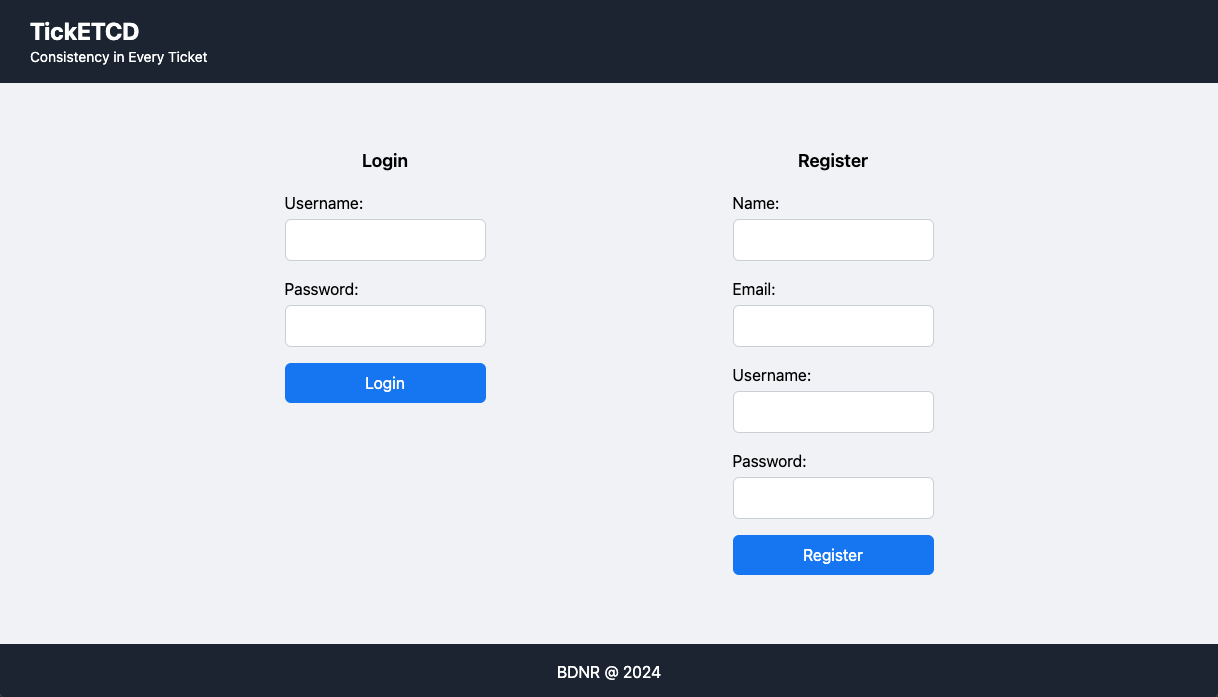
\includegraphics[width=1\textwidth]{login.png}
        \caption{Login/register page, where a user can register if not have a account yet or login in their account.}
        \label{fig:login}
    \end{figure}

\hspace{1cm}

\pagebreak
\hspace{1cm}

    \begin{figure}[h!]
        \centering
        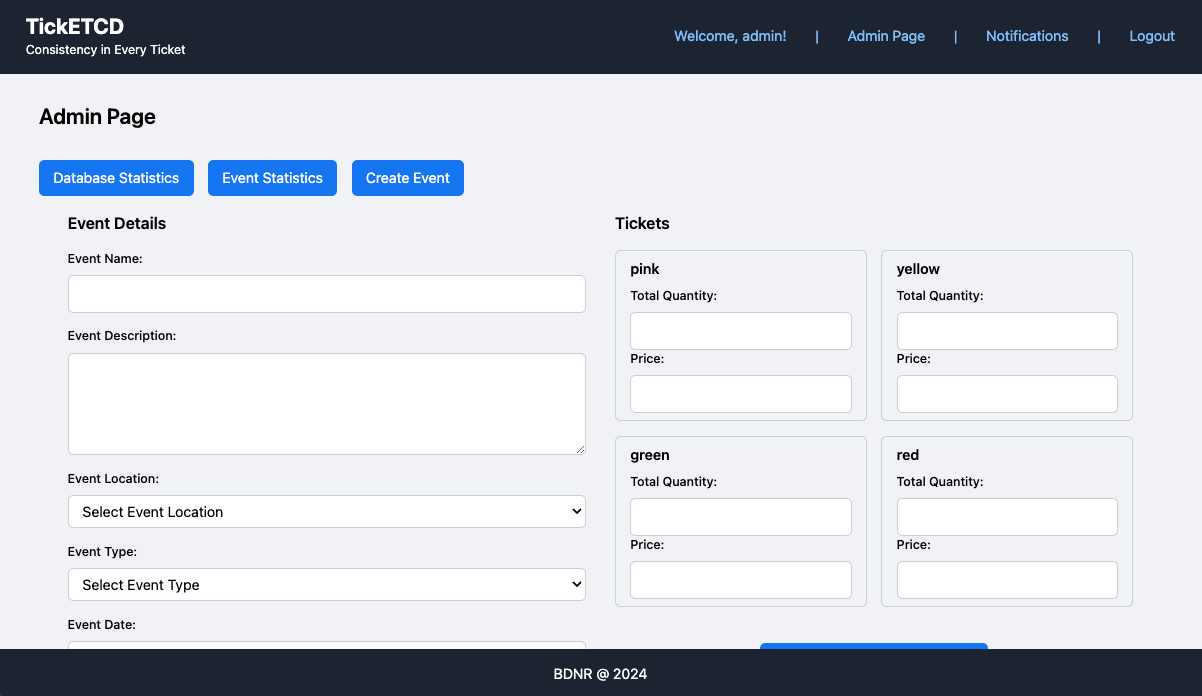
\includegraphics[width=1\textwidth]{admin-event.png}
        \caption{Admin page for creation of a new event in the platform.}
        \label{fig:admin-event}
    \end{figure}

\hspace{1cm}

\hspace{1cm}

    \begin{figure}[h!]
        \centering
        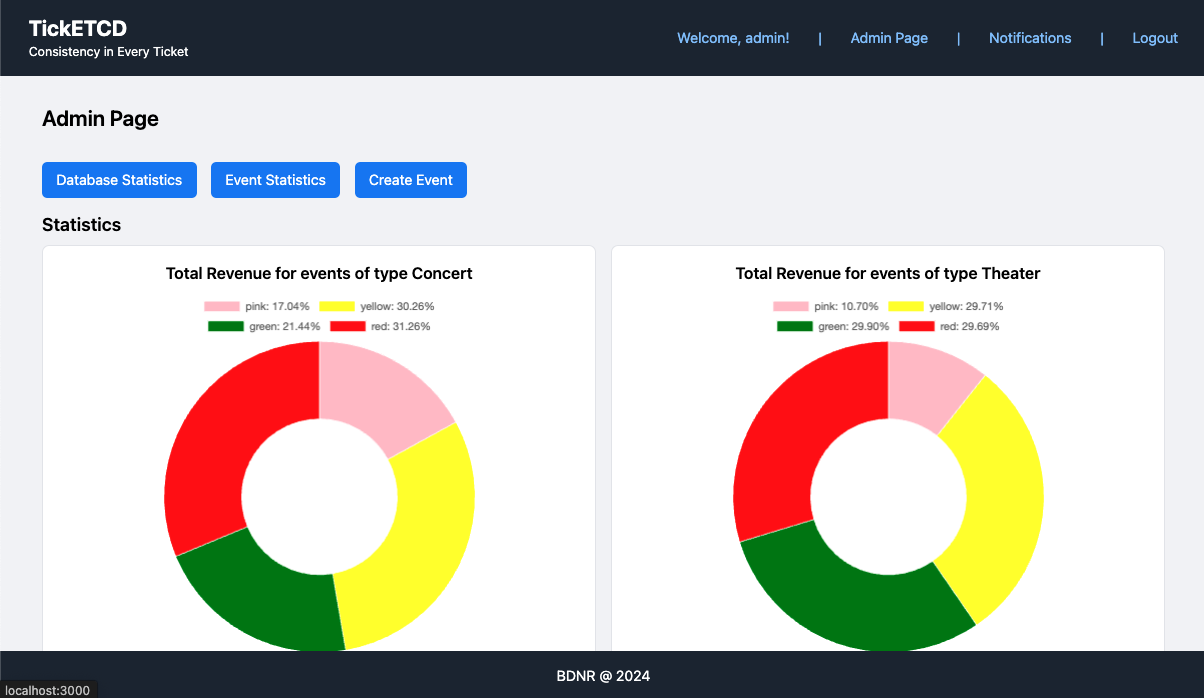
\includegraphics[width=1\textwidth]{admin-statistics.png}
        \caption{Admin page showing the statistics about the events in the platform.}
        \label{fig:admin-statistics}
    \end{figure}

\hspace{1cm}
\pagebreak
\hspace{1cm}

    \begin{figure}[h!]
        \centering
        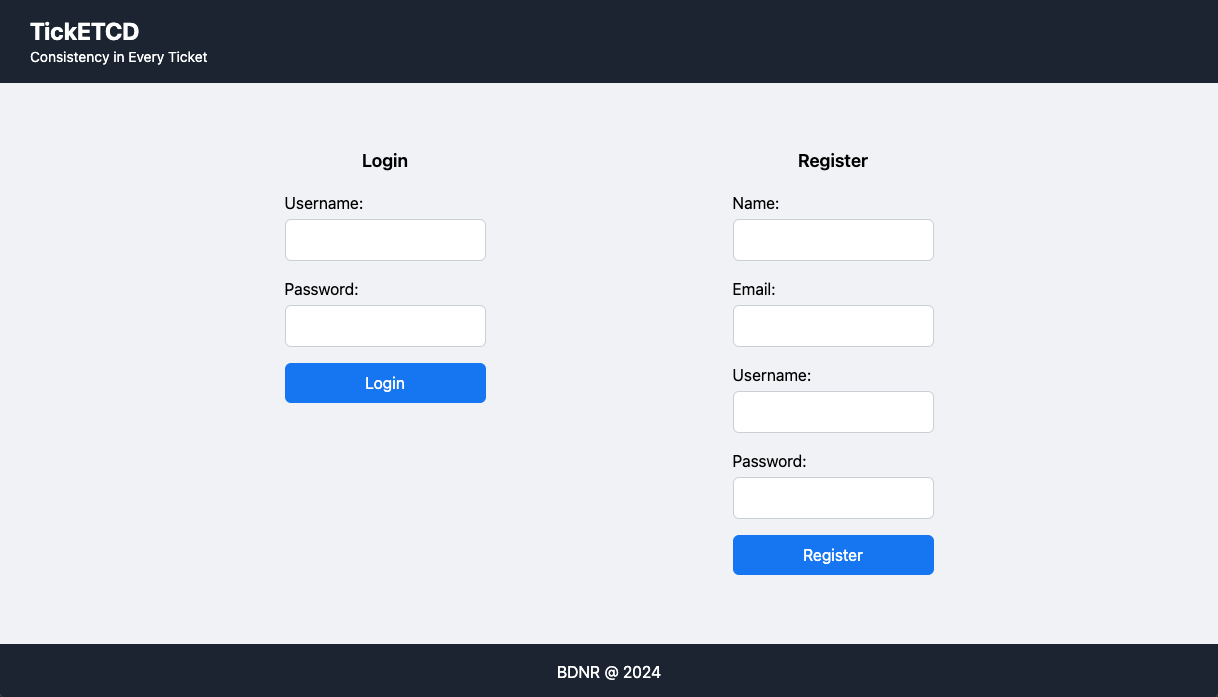
\includegraphics[width=1\textwidth]{login.png}
        \caption{Login/register page, where a user can register if not have a account yet or login in their account.}
        \label{fig:login}
    \end{figure}

\hspace{1cm}


\hspace{1cm}

    \begin{figure}[h!]
        \centering
        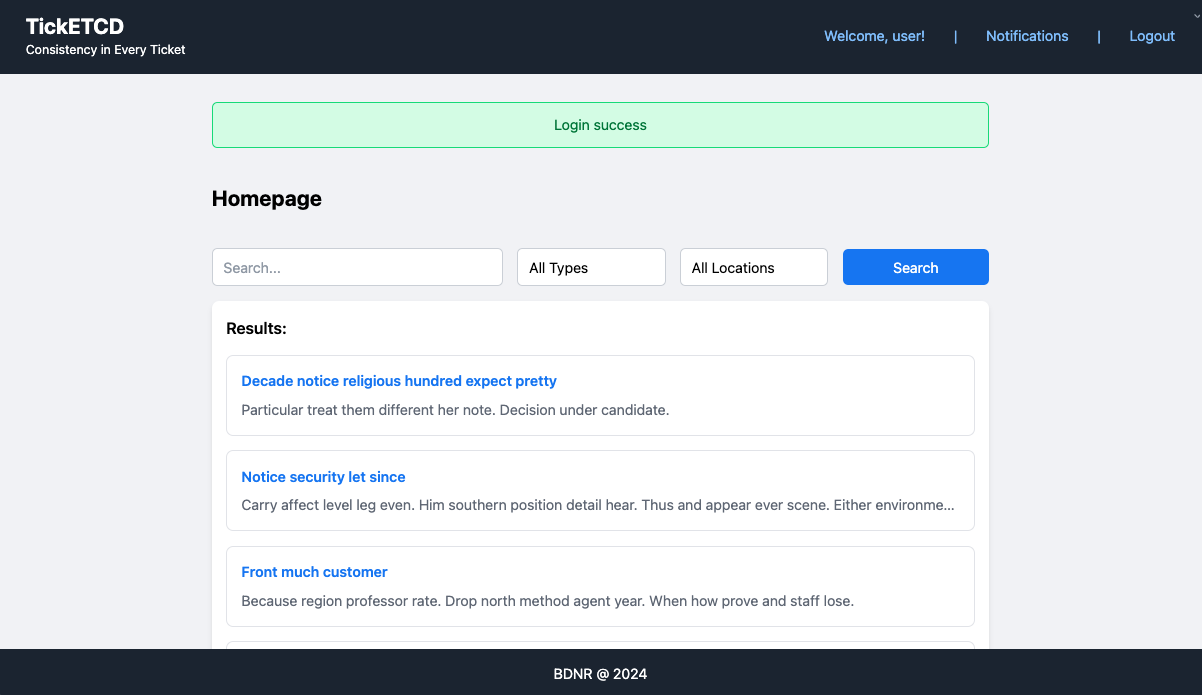
\includegraphics[width=1\textwidth]{home.png}
        \caption{Home page, where a user can search for a certain event.}
        \label{fig:home}
    \end{figure}

\hspace{1cm}
\pagebreak
\hspace{1cm}

    \begin{figure}[h!]
        \centering
        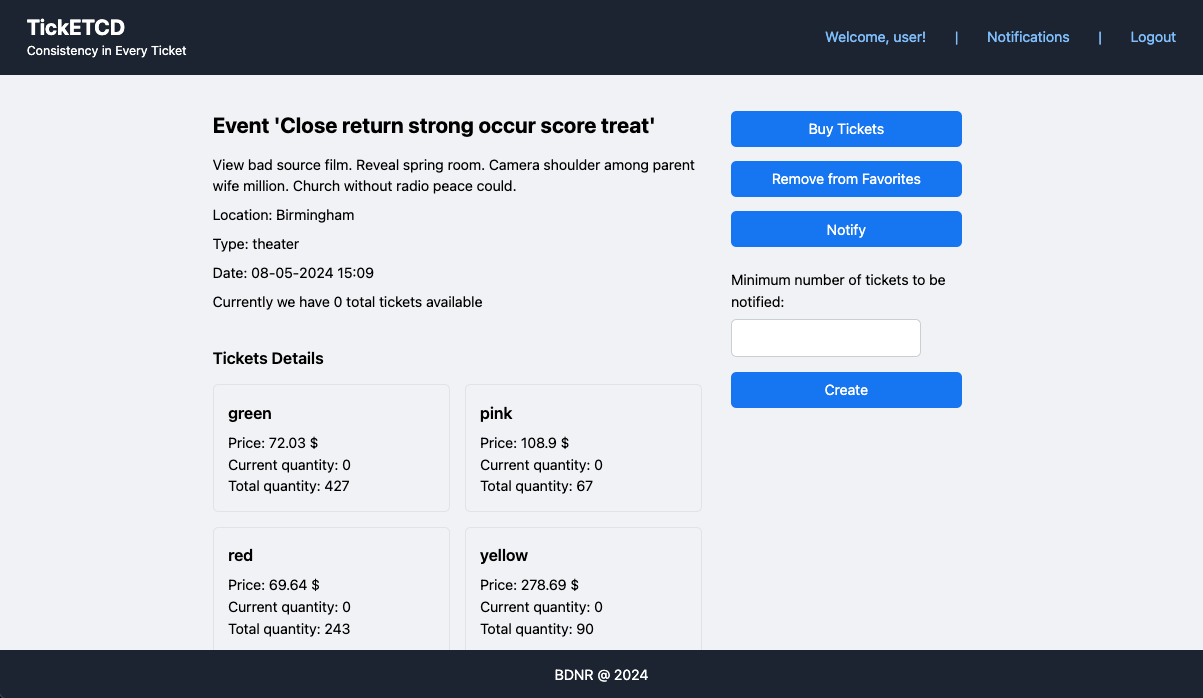
\includegraphics[width=1\textwidth]{event.png}
        \caption{Event page, where a user can see the details about a certain event, buy tickets, add that event to favourite or be notify when that event has less than x tickets.}
        \label{fig:event}
    \end{figure}

\hspace{1cm}

\hspace{1cm}

    \begin{figure}[h!]
        \centering
        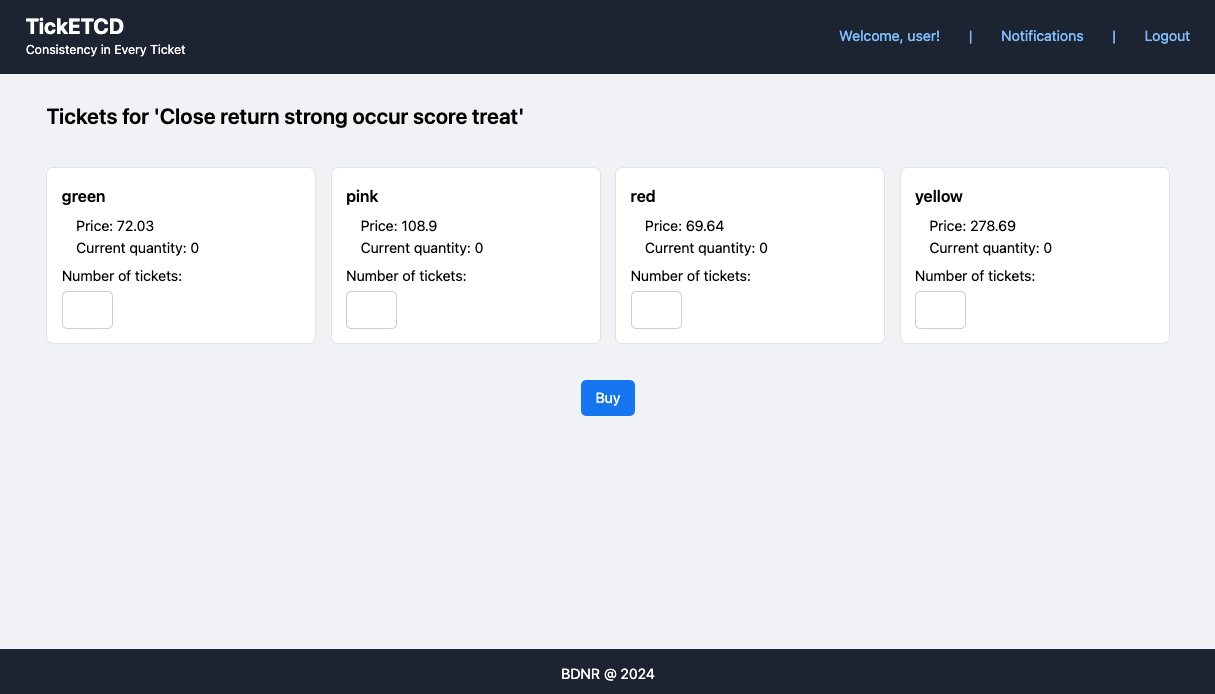
\includegraphics[width=1\textwidth]{buy.png}
        \caption{Purchase page, where the user can select the number of tickets they want to buy of each type.}
        \label{fig:buy}
    \end{figure}

\hspace{1cm}
\pagebreak
\hspace{1cm}

    \begin{figure}[h!]
        \centering
        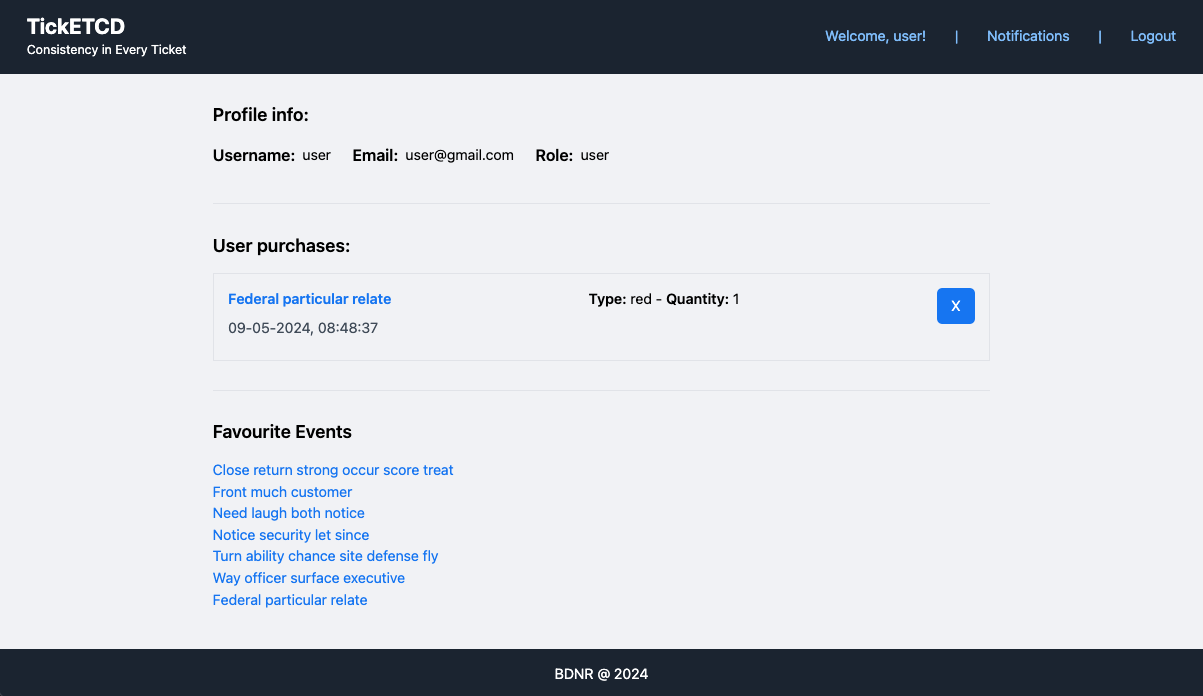
\includegraphics[width=1\textwidth]{profile.png}
        \caption{Profile page, where user can see the information about themselves, the events that they marked as favourite, the historic about the purchases done and cancel them.}
        \label{fig:profile}
    \end{figure}

\hspace{1cm}

\hspace{1cm}

    \begin{figure}[h!]
        \centering
        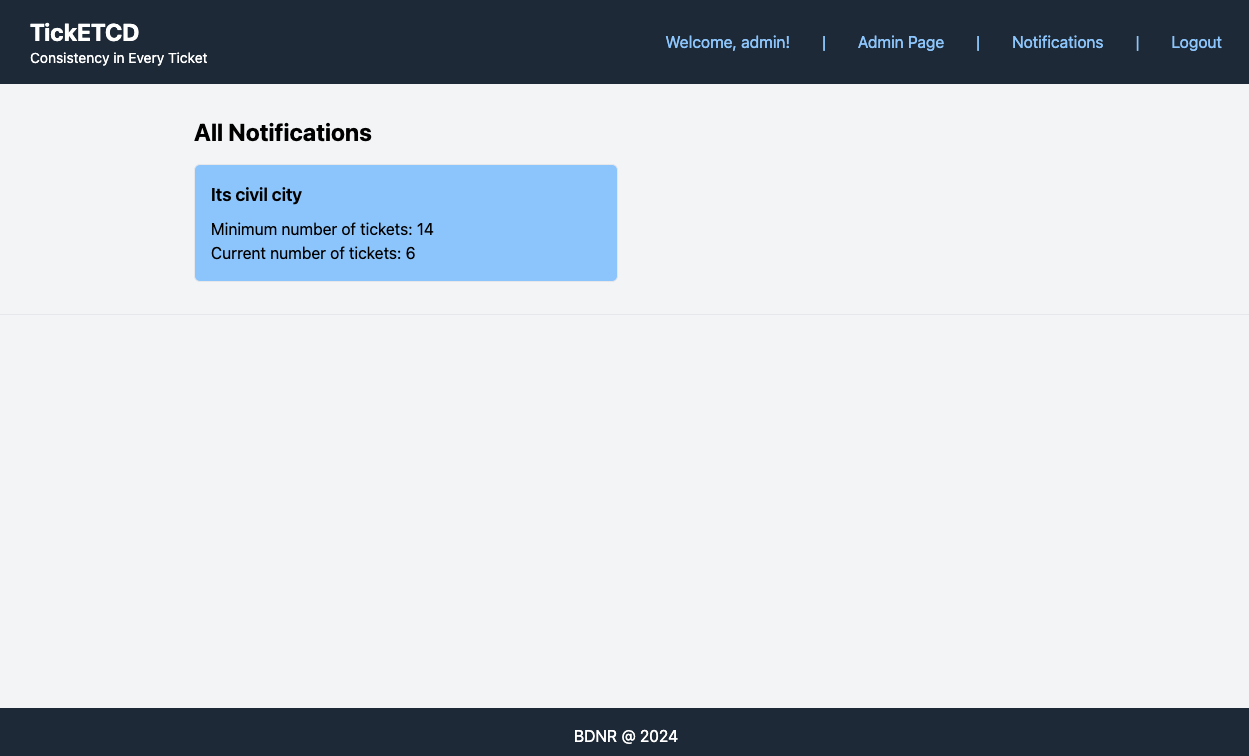
\includegraphics[width=1\textwidth]{notifications.png}
        \caption{Notifications page, where user can see all the notifications that they created, the ones that are active and the ones that are not.}
        \label{fig:notification}
    \end{figure}

\hspace{1cm}
\pagebreak

%% The next two lines define the bibliography style to be used, and
%% the bibliography file.
\nocite{*}
\def\BibTex{BibTeX}
\bibliographystyle{ACM-Reference-Format}
\bibliography{sample-base}

\end{document}
\endinput
%%
%% End of file `sample-manuscript.tex'.
